\documentclass[11pt,a4paper]{article}
\usepackage[utf8]{inputenc}
\usepackage[T1]{fontenc}
\usepackage{graphicx}
\usepackage{amsmath}
\usepackage{amssymb}
\usepackage{hyperref}
\usepackage{booktabs}
\usepackage{geometry}
\usepackage{float}
\usepackage{xcolor}
\usepackage{listings}
\usepackage{caption}

\geometry{margin=1in}
\hypersetup{colorlinks=true, linkcolor=blue, urlcolor=blue, citecolor=blue}

\title{ Evaluation Test: DeepLense \\
PyTorch Implementations for Gravitational Lensing Findings}
\author{Prabesh Aryal}
\date{\today}

\begin{document}

\maketitle

\begin{abstract}
This report details the methodologies and results for the DeepLense Gravitational Lens Finding evaluation test, encompassing both multi-class and binary classification tasks. For Task 1, we implemented a Convolutional Neural Network (CNN) in PyTorch to classify astronomical images into three classes: no substructure, subhalo substructure, and vortex substructure. Despite employing a balanced dataset and standard CNN architecture, the multi-class model achieved limited success. For Task 2, we addressed the binary classification of gravitational lenses versus non-lensed galaxies, tackling the significant challenge of class imbalance. By utilizing class weighting and regularization within a similar CNN framework, we attained an AUC score of 0.9488 on a highly imbalanced test set (1:100 ratio), demonstrating robust lens detection capabilities. Implementation details, model weights, and complete code are available in our GitHub repository: \url{https://github.com/prabeshAryal/gravitational-lensing-problem}.
\end{abstract}

\section{Introduction}
Strong gravitational lensing, a phenomenon predicted by Einstein's theory of general relativity, occurs when light from a distant source is deflected by the gravitational field of a massive intervening object, such as a galaxy or galaxy cluster. This effect can create distinctive visual signatures like multiple images, arcs, or Einstein rings, observable in astronomical surveys. The automated identification of these lensing events is vital for advancing our understanding of dark matter distribution and the formation of cosmic structures.

This evaluation test explores two distinct but related tasks: multi-class classification of lens substructure types and binary classification of lensed versus non-lensed galaxies. Both tasks present unique challenges. Multi-class classification requires differentiating subtle visual features across multiple categories, while binary classification in realistic scenarios suffers from extreme class imbalance, reflecting the rarity of strong lensing events in astronomical observations. This report outlines our approach, results, and discussions for both tasks, aiming to develop robust deep learning models capable of identifying gravitational lensing phenomena from astronomical images.

\section{Task 1: Multi-Class Classification}

\subsection{Dataset}
The dataset for Task 1 comprises three classes of astronomical images: 'no substructure', 'subhalo substructure', and 'vortex substructure'. Each image is a 3-channel representation of size $64 \times 64$ pixels. The dataset is balanced across the three classes to facilitate multi-class classification without initial concerns of class imbalance. The dataset statistics are as follows:

\begin{itemize}
    \item Training dataset: 10,000 images per class (30,000 total)
    \item Validation dataset: 2,500 images per class (7,500 total)
    \item Test dataset: 2,500 images per class (7,500 total)
\end{itemize}

\begin{figure}[H]
    \centering
    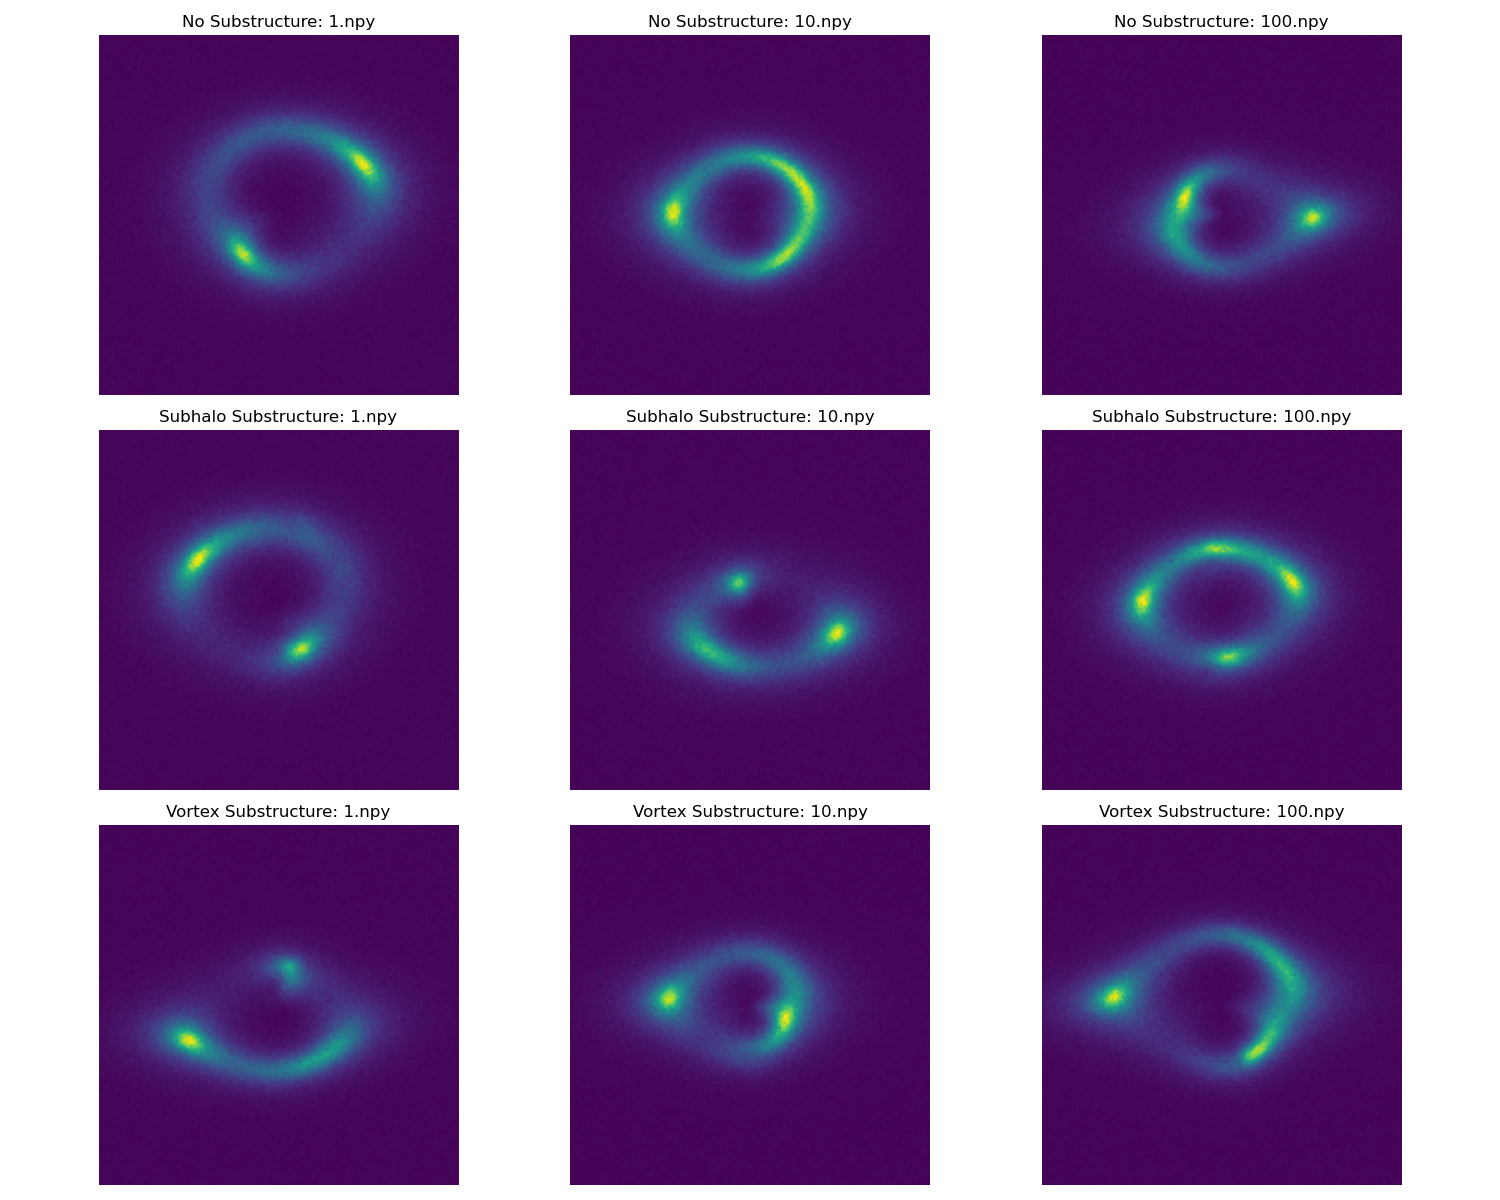
\includegraphics[width=0.7\textwidth]{../Task1/results/sample_images_multi.png}
    \caption{Sample images from the Task 1 dataset: no substructure, subhalo substructure, and vortex substructure (from top to bottom rows).}
    \label{fig:sample_images_multi}
\end{figure}

\subsection{Methodology}

\subsubsection{Data Preprocessing}
For Task 1, each image was normalized by subtracting the channel-wise mean and dividing by the channel-wise standard deviation. This normalization was applied to both training and validation datasets to ensure stable and efficient training. The provided dataset was already split into training and validation sets, which were used as provided.

\subsubsection{Model Architecture}
We implemented a Convolutional Neural Network (CNN) specifically designed for multi-class classification. The architecture consists of four convolutional blocks, each sequentially arranged as follows:

\begin{itemize}
    \item Convolutional layer (with 32, 64, 128, and 256 filters respectively)
    \item Batch normalization
    \item ReLU activation
    \item Max pooling (2×2)
    \item Dropout (rate=0.5) for regularization
\end{itemize}

These convolutional blocks are followed by two fully connected layers (512 neurons in the hidden layer) and a final output layer to produce logits for the three classes. Dropout is also applied in the fully connected layers to further prevent overfitting.

The detailed architecture is as follows:
\begin{itemize}
    \item Input: 3×64×64 (multi-filter image)
    \item Conv1: 32 filters, 3×3 kernel, padding=1 $\rightarrow$ 32×64×64
    \item BatchNorm1 + ReLU + MaxPool $\rightarrow$ 32×32×32
    \item Dropout (0.5)
    \item Conv2: 64 filters, 3×3 kernel, padding=1 $\rightarrow$ 64×32×32
    \item BatchNorm2 + ReLU + MaxPool $\rightarrow$ 64×16×16
    \item Dropout (0.5)
    \item Conv3: 128 filters, 3×3 kernel, padding=1 $\rightarrow$ 128×16×16
    \item BatchNorm3 + ReLU + MaxPool $\rightarrow$ 128×8×8
    \item Dropout (0.5)
    \item Conv4: 256 filters, 3×3 kernel, padding=1 $\rightarrow$ 256×8×8
    \item BatchNorm4 + ReLU + MaxPool $\rightarrow$ 256×4×4
    \item Dropout (0.5)
    \item Flatten $\rightarrow$ 4096
    \item FC1: 4096 $\rightarrow$ 512 + ReLU
    \item Dropout (0.5)
    \item FC2: 512 $\rightarrow$ 3 (output logits)
\end{itemize}
The PyTorch implementation of this architecture is available in the GitHub repository.

\subsubsection{Training Strategy}
The model for Task 1 was trained for 25 epochs using the Adam optimizer with a learning rate of $10^{-3}$ and weight decay of $10^{-4}$.  CrossEntropyLoss was used as the loss function, and a ReduceLROnPlateau learning rate scheduler was employed to reduce the learning rate by a factor of 0.5 if the validation loss plateaued for 3 epochs. Model weights were saved whenever validation loss improved.

\subsection{Results}

\subsubsection{Training Performance}
During training, the model demonstrated initial fluctuations in loss and accuracy but did not show substantial improvement over epochs, especially in validation metrics. The training logs illustrate this behavior:

\begin{table}[H]
    \centering
    \caption{Training and validation metrics for Task 1 across epochs}
    \label{tab:training_metrics_multi}
    \begin{tabular}{ccccc}
    \toprule
    \textbf{Epoch} & \textbf{Train Loss} & \textbf{Train Acc (\%)} & \textbf{Val Loss} & \textbf{Val Acc (\%)} \\
    \midrule
    1 & 1.1629 & 33.51 & 1.0987 & 33.33 \\
    2 & 1.0994 & 33.35 & 1.0986 & 33.33 \\
    3 & 1.0999 & 32.94 & 1.0986 & 33.33 \\
    4 & 1.0995 & 33.12 & 1.0987 & 33.33 \\
    ... & ... & ... & ... & ... \\
    23 & 1.0989 & 33.74 & 1.0984 & 33.48 \\
    24 & 1.0988 & 33.64 & 1.0985 & 34.00 \\
    25 & 1.0991 & 34.04 & 1.0985 & 34.19 \\
    \bottomrule
    \end{tabular}
\end{table}
\textit{Note: Only a subset of epochs is displayed in the table. Refer to the console output logs for complete data.}

The table and the training history plot indicate that the model struggled to learn meaningful features to differentiate between the three classes, as the validation accuracy remained consistently around chance level ($\sim$33\% for a 3-class problem).

\begin{figure}[H]
    \centering
    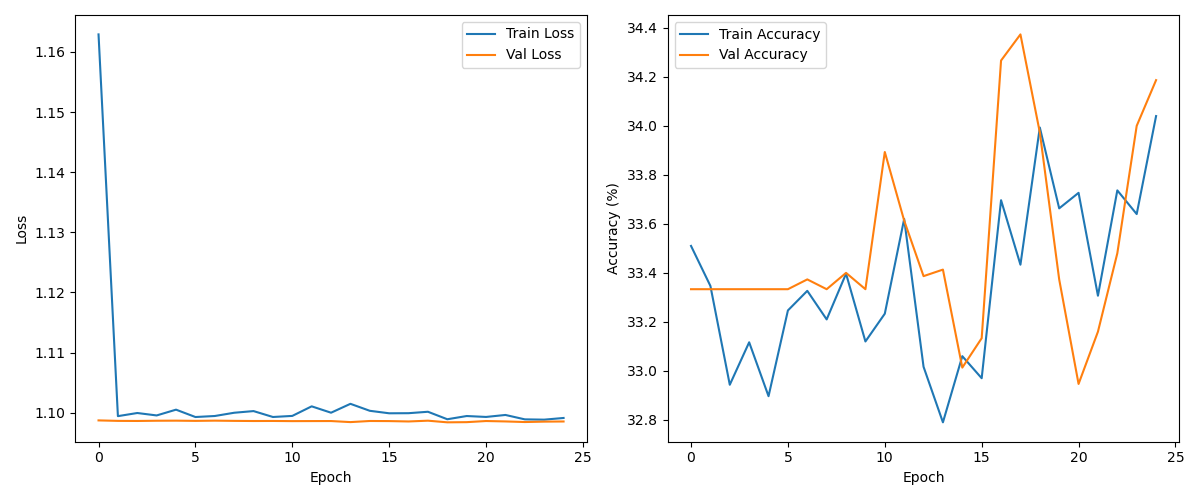
\includegraphics[width=0.7\textwidth]{../Task1/results/training_history_multi.png}
    \caption{Training and validation metrics over epochs for Task 1.}
    \label{fig:training_history_multi}
\end{figure}

\subsubsection{Classification Performance}
The classification performance for Task 1 is poor, as evidenced by the ROC curves, confusion matrix, and classification report. The weighted average AUC score is 0.5086, close to random guessing.

\begin{figure}[H]
    \centering
    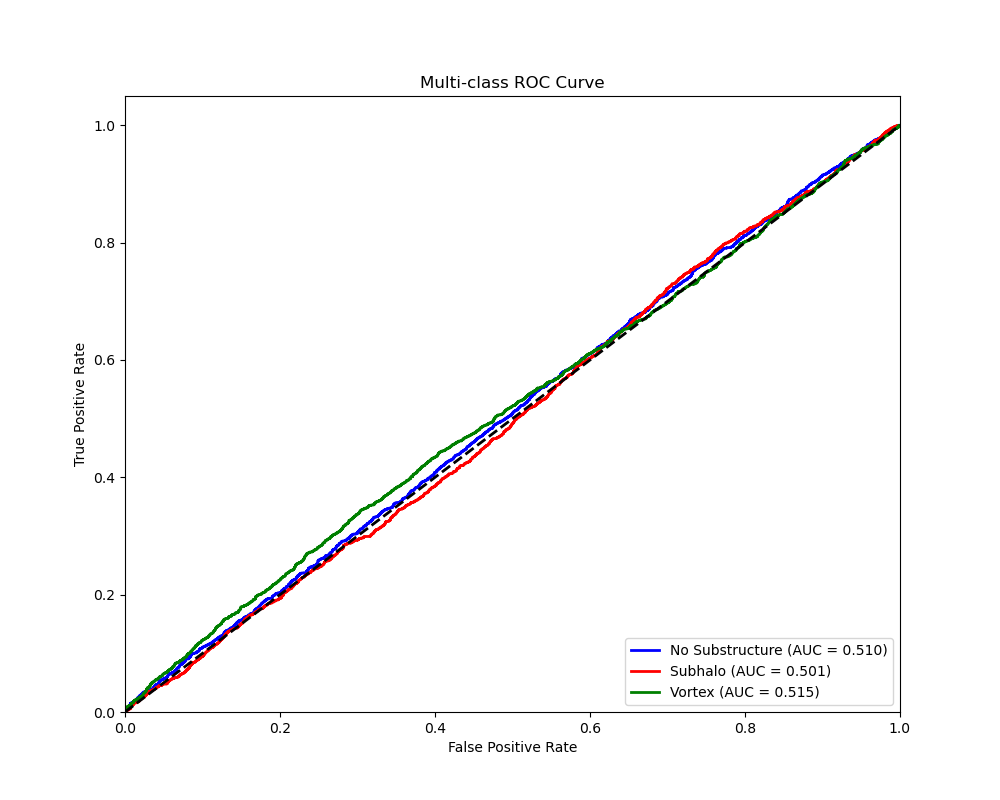
\includegraphics[width=0.6\textwidth]{../Task1/results/roc_curve_multi.png}
    \caption{ROC curve for Task 1 showing near-random performance with a weighted AUC score of 0.5086.}
    \label{fig:roc_curve_multi}
\end{figure}

\begin{figure}[H]
    \centering
    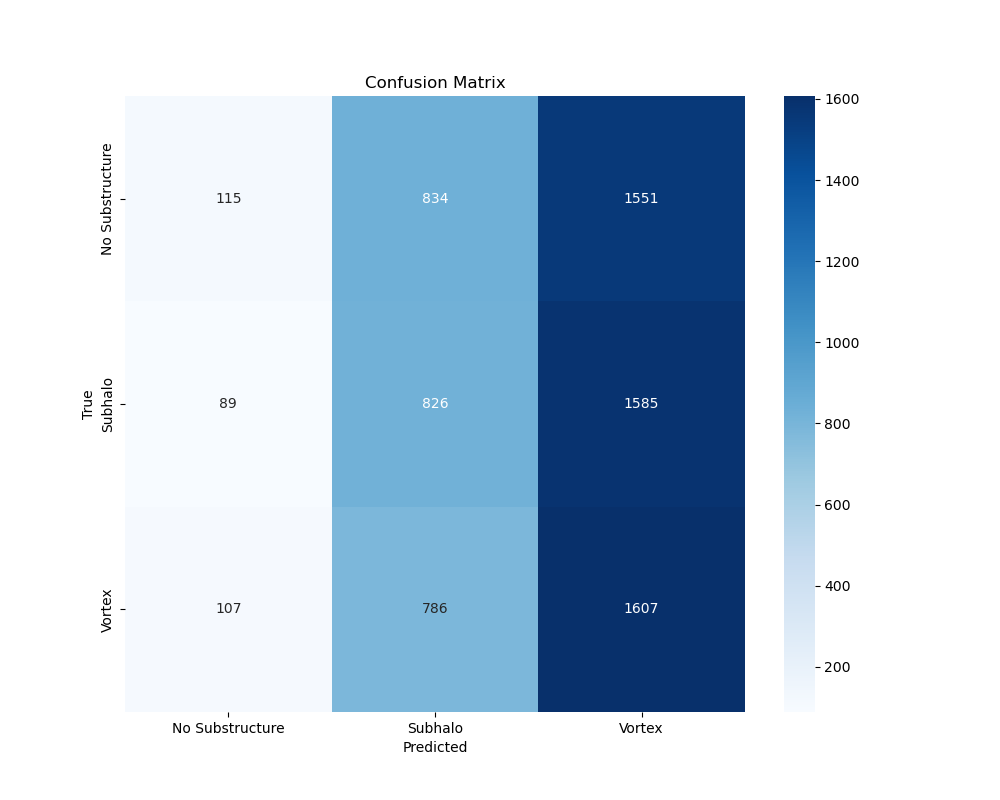
\includegraphics[width=0.6\textwidth]{../Task1/results/confusion_matrix_multi.png}
    \caption{Confusion matrix for Task 1, indicating poor classification performance across all classes.}
    \label{fig:confusion_matrix_multi}
\end{figure}

The detailed classification report further underscores the lack of discriminative capability:

\begin{table}[H]
    \centering
    \caption{Classification performance metrics for Task 1}
    \label{tab:classification_report_multi}
    \begin{tabular}{ccccc}
    \toprule
    \textbf{Class} & \textbf{Precision} & \textbf{Recall} & \textbf{F1-score} & \textbf{Support} \\
    \midrule
    No Substructure (0) & 0.37 & 0.05 & 0.08 & 2500 \\
    Subhalo (1) & 0.34 & 0.33 & 0.33 & 2500 \\
    Vortex (2) & 0.34 & 0.64 & 0.44 & 2500 \\
    \midrule
    Accuracy & & & 0.34 & 7500 \\
    Macro avg & 0.35 & 0.34 & 0.29 & 7500 \\
    Weighted avg & 0.35 & 0.34 & 0.29 & 7500 \\
    \bottomrule
    \end{tabular}
\end{table}

\begin{figure}[H]
    \centering
    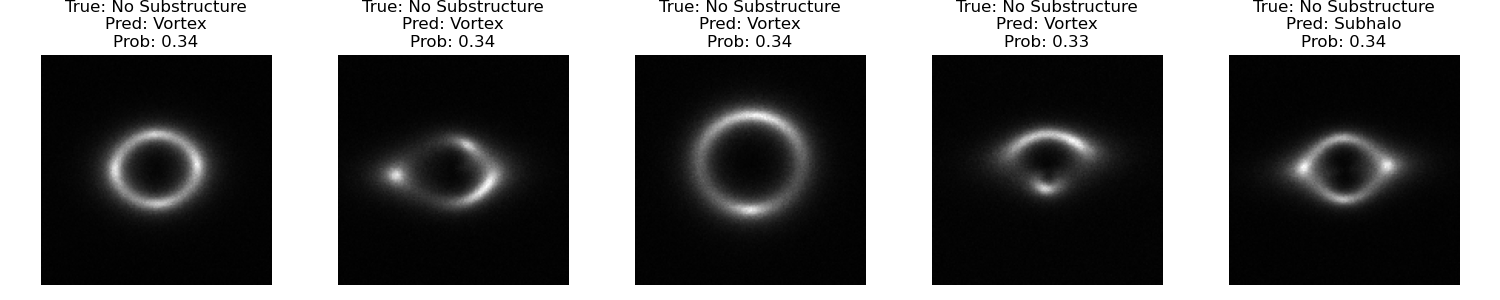
\includegraphics[width=0.9\textwidth]{../Task1/results/sample_predictions_multi.png}
    \caption{Sample predictions from Task 1 showing low confidence and frequent misclassifications.}
    \label{fig:sample_predictions_multi}
\end{figure}

\subsection{Discussion on Task 1}
The results for Task 1 indicate that the implemented CNN model, with the current architecture and training configuration, fails to effectively classify the three types of substructures. The near-chance level AUC score and accuracy suggest that the model is not learning to distinguish relevant features for multi-class classification within the given number of epochs and model complexity.

Possible reasons for the poor performance could include:

\begin{itemize}
    \item \textbf{Subtlety of Features}: The visual differences between the three classes might be very subtle, requiring a more complex model architecture or enhanced feature extraction techniques.
    \item \textbf{Model Capacity}: The current CNN architecture might not be deep or wide enough to capture the necessary discriminative features for this multi-class problem.
    \item \textbf{Training Regimen}:  While standard training procedures were followed, hyperparameters such as learning rate, weight decay, or the number of epochs might need further optimization. Data augmentation could also potentially improve the model's ability to generalize.
\end{itemize}

\subsection{Conclusion for Task 1}
In conclusion, the CNN model implemented for Task 1, aimed at multi-class classification of gravitational lens substructures, did not achieve satisfactory performance. The model's inability to surpass chance-level accuracy suggests that more sophisticated approaches may be needed to effectively tackle this classification problem. Future work could explore deeper and more complex CNN architectures, investigate different training strategies, or incorporate techniques to enhance the subtle visual features distinguishing the classes.


\section{Task 2: Binary Classification}

\subsection{Dataset}
The dataset for Task 2 is designed for binary classification: distinguishing between lensed and non-lensed galaxies. Each object is represented as a 3-channel image of size $64 \times 64$ pixels, corresponding to different SDSS filters. The key characteristic of this dataset is its class imbalance, particularly in the test set, which mirrors the rarity of lensing events in astronomical surveys. The dataset statistics are as follows:

\begin{itemize}
    \item Training dataset: 1,730 lensed and 28,675 non-lensed galaxies (ratio of approximately 1:17)
    \item Test dataset: 195 lensed and 19,455 non-lensed galaxies (ratio of approximately 1:100)
    \item Training/validation split: 27,364 training (90\%) and 3,041 validation (10\%) samples
\end{itemize}

This imbalance reflects the reality of astronomical observations, where strong gravitational lensing is a rare phenomenon. The test set distribution is particularly skewed, presenting a more realistic scenario for model evaluation in actual survey conditions.

\begin{figure}[H]
    \centering
    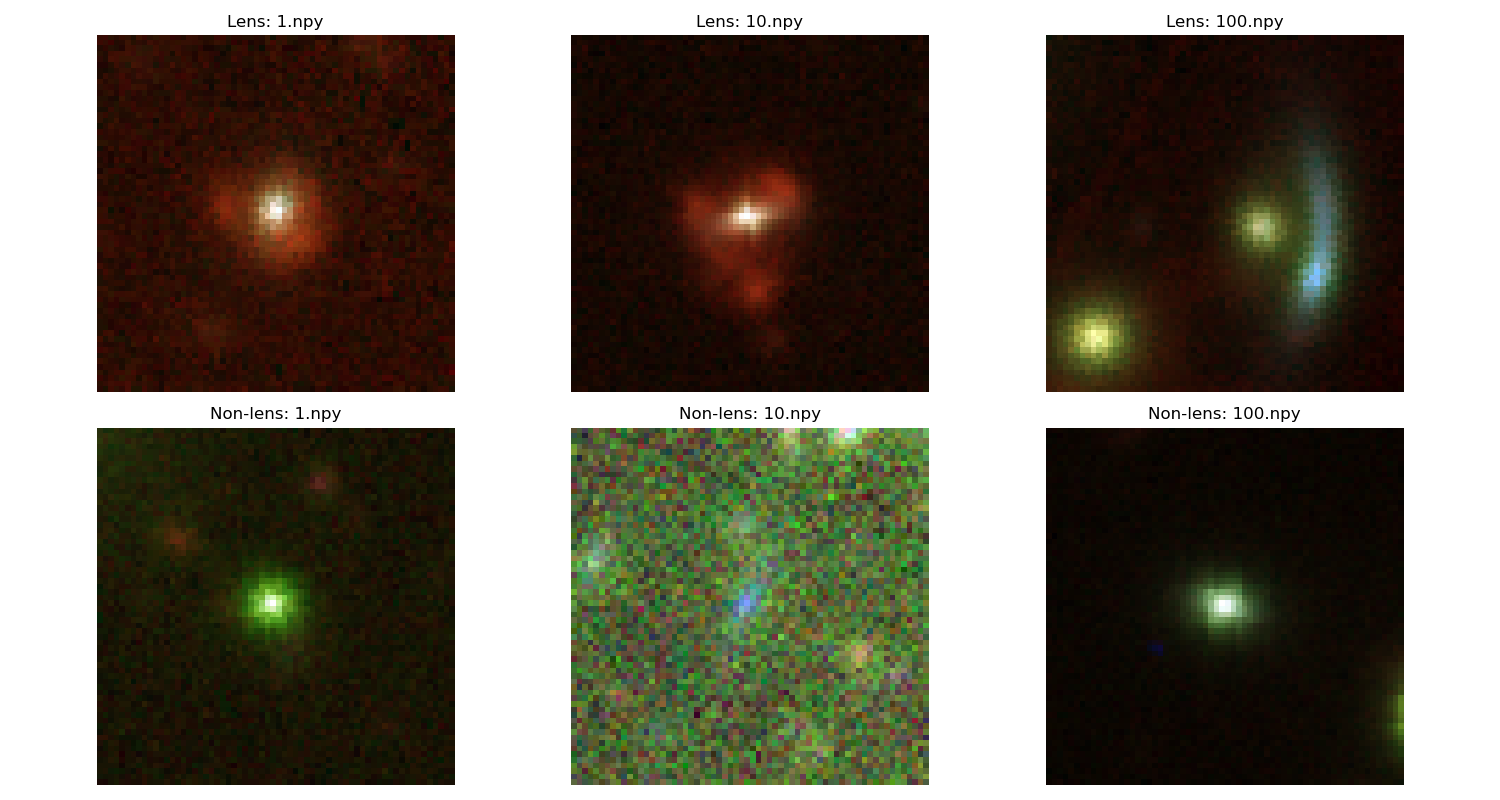
\includegraphics[width=0.8\textwidth]{../Task2/results/sample_images.png}
    \caption{Sample images from the Task 2 dataset: lensed galaxies (top row) and non-lensed galaxies (bottom row).}
    \label{fig:sample_images}
\end{figure}

\subsection{Methodology}

\subsubsection{Data Preprocessing}
Similar to Task 1, each image in Task 2 was normalized by subtracting the mean and dividing by the standard deviation channel-wise. This normalization ensures stable training and helps the model learn effectively across different filter bands. The dataset was split into training, validation, and test sets as described in the dataset description.

\subsubsection{Model Architecture}
The CNN architecture for Task 2 consists of three convolutional blocks, each containing:
\begin{itemize}
    \item Convolutional layer (with 32, 64, and 128 filters respectively)
    \item Batch normalization
    \item ReLU activation
    \item Max pooling (2×2)
    \item Dropout (rate=0.5) for regularization
\end{itemize}

Following the convolutional layers are two fully connected layers (with 512 neurons in the hidden layer) and dropout for classification.

The complete architecture is as follows:
\begin{itemize}
    \item Input: 3×64×64 (multi-filter image)
    \item Conv1: 32 filters, 3×3 kernel, padding=1 $\rightarrow$ 32×64×64
    \item BatchNorm1 + ReLU + MaxPool $\rightarrow$ 32×32×32
    \item Dropout (0.5)
    \item Conv2: 64 filters, 3×3 kernel, padding=1 $\rightarrow$ 64×32×32
    \item BatchNorm2 + ReLU + MaxPool $\rightarrow$ 64×16×16
    \item Dropout (0.5)
    \item Conv3: 128 filters, 3×3 kernel, padding=1 $\rightarrow$ 128×16×16
    \item BatchNorm3 + ReLU + MaxPool $\rightarrow$ 128×8×8
    \item Dropout (0.5)
    \item Flatten $\rightarrow$ 8192
    \item FC1: 8192 $\rightarrow$ 512 + ReLU
    \item Dropout (0.5)
    \item FC2: 512 $\rightarrow$ 2 (output logits)
\end{itemize}

\subsubsection{Training Strategy}
To address the class imbalance, class weights were implemented in the loss function, giving higher importance to the minority class (lensed galaxies). The weights were calculated as:

\begin{equation}
    w_c = \frac{N_{total}}{2 \times N_c}
\end{equation}

where $N_{total}$ is the total number of samples and $N_c$ is the number of samples in class $c$.

The model was trained for 20 epochs using Adam optimizer with a learning rate of $10^{-3}$ and weight decay of $10^{-4}$. A learning rate scheduler (ReduceLROnPlateau) was used to reduce the learning rate by a factor of 0.5 when validation performance plateaued for 3 consecutive epochs. The model weights were saved at epochs with improved validation performance.

\subsection{Results}

\subsubsection{Training Performance}
The model showed steady improvement during training, with both loss and accuracy metrics indicating good convergence. Full training logs show the progression across all 20 epochs in Table \ref{tab:training_metrics}.

\begin{table}[H]
    \centering
    \caption{Training and validation metrics across all epochs for Task 2}
    \label{tab:training_metrics}
    \begin{tabular}{ccccc}
    \toprule
    \textbf{Epoch} & \textbf{Train Loss} & \textbf{Train Acc (\%)} & \textbf{Val Loss} & \textbf{Val Acc (\%)} \\
    \midrule
    1 & 0.6849 & 75.10 & 0.5469 & 63.60 \\
    2 & 0.5319 & 76.82 & 0.4226 & 84.22 \\
    3 & 0.4952 & 79.68 & 0.3509 & 83.33 \\
    4 & 0.4481 & 82.47 & 0.3897 & 92.31 \\
    5 & 0.4468 & 83.23 & 0.3345 & 90.53 \\
    6 & 0.4330 & 83.50 & 0.3049 & 87.80 \\
    7 & 0.3987 & 86.14 & 0.2835 & 91.35 \\
    8 & 0.3720 & 86.20 & 0.3486 & 82.83 \\
    9 & 0.3859 & 85.76 & 0.3034 & 85.76 \\
    10 & 0.3624 & 86.45 & 0.2800 & 89.44 \\
    11 & 0.3651 & 86.59 & 0.2648 & 90.04 \\
    12 & 0.3544 & 86.87 & 0.2510 & 88.19 \\
    13 & 0.3578 & 87.24 & 0.3844 & 94.87 \\
    14 & 0.3865 & 87.02 & 0.2959 & 86.12 \\
    15 & 0.3792 & 86.98 & 0.2676 & 88.92 \\
    16 & 0.3449 & 86.95 & 0.2364 & 90.43 \\
    17 & 0.3575 & 86.94 & 0.2474 & 92.27 \\
    18 & 0.3447 & 87.44 & 0.2667 & 88.42 \\
    19 & 0.3341 & 87.40 & 0.2591 & 86.48 \\
    20 & 0.3373 & 87.55 & 0.2548 & 92.63 \\
    \bottomrule
    \end{tabular}
\end{table}

\begin{figure}[H]
    \centering
    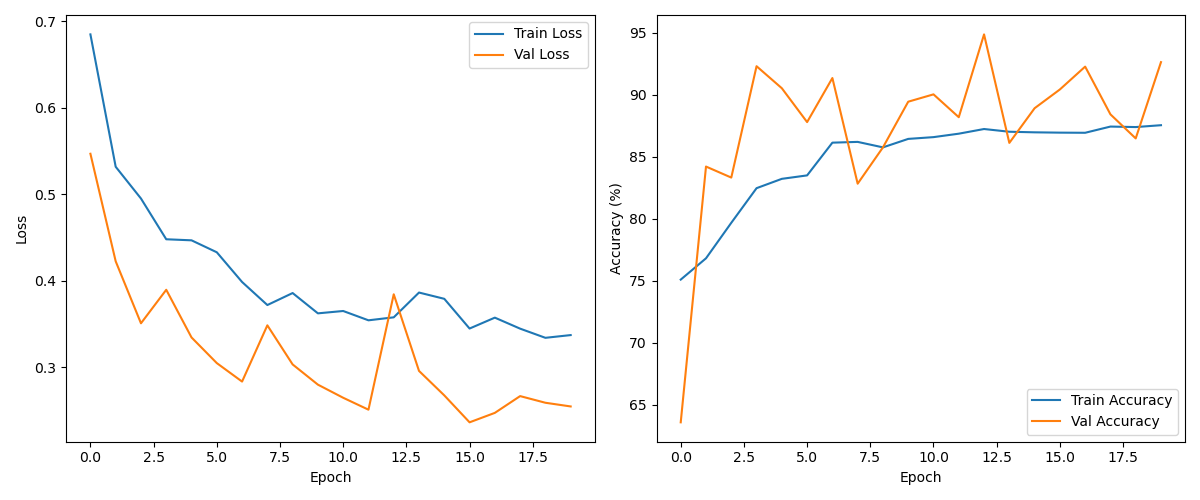
\includegraphics[width=0.8\textwidth]{../Task2/results/training_history.png}
    \caption{Training and validation metrics over epochs for Task 2.}
    \label{fig:training_history}
\end{figure}

\subsubsection{Classification Performance}

The model achieved high classification performance for Task 2 as evidenced by the ROC curve and confusion matrix. The final AUC score was 0.9488, indicating excellent discriminative ability between lensed and non-lensed galaxies.

\begin{figure}[H]
    \centering
    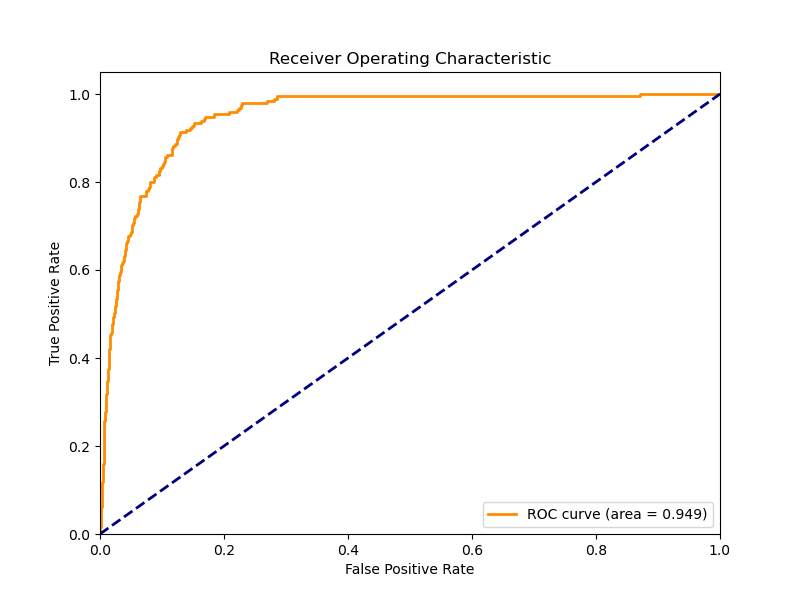
\includegraphics[width=0.6\textwidth]{../Task2/results/roc_curve.png}
    \caption{ROC curve showing model performance for Task 2 with AUC score of 0.9488.}
    \label{fig:roc_curve}
\end{figure}

\begin{figure}[H]
    \centering
    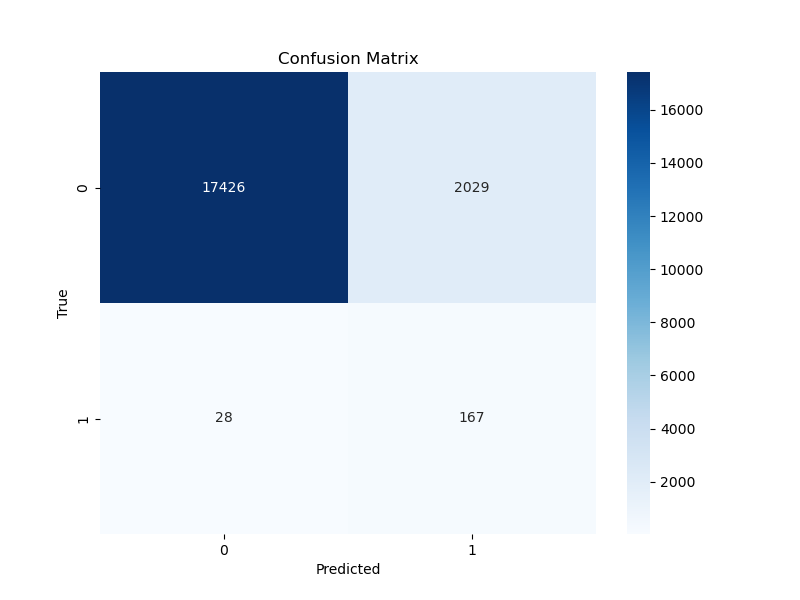
\includegraphics[width=0.6\textwidth]{../Task2/results/confusion_matrix.png}
    \caption{Confusion matrix displaying the model's classification performance for Task 2.}
    \label{fig:confusion_matrix}
\end{figure}

The detailed classification report is presented below:

\begin{table}[H]
    \centering
    \caption{Classification performance metrics for Task 2}
    \label{tab:classification_report}
    \begin{tabular}{ccccc}
    \toprule
    \textbf{Class} & \textbf{Precision} & \textbf{Recall} & \textbf{F1-score} & \textbf{Support} \\
    \midrule
    Non-lensed (0) & 1.00 & 0.90 & 0.94 & 19,455 \\
    Lensed (1) & 0.08 & 0.86 & 0.14 & 195 \\
    \midrule
    Accuracy & & & 0.90 & 19,650 \\
    Macro avg & 0.54 & 0.88 & 0.54 & 19,650 \\
    Weighted avg & 0.99 & 0.90 & 0.94 & 19,650 \\
    \bottomrule
    \end{tabular}
\end{table}

\begin{figure}[H]
    \centering
    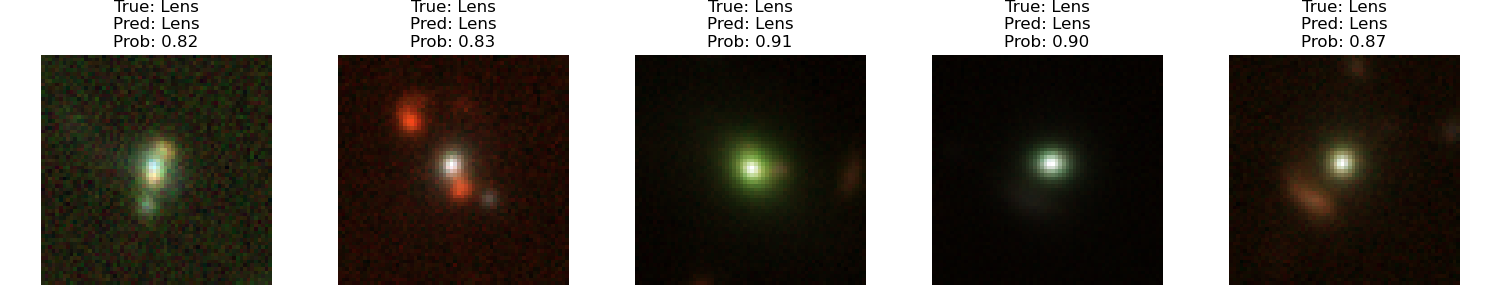
\includegraphics[width=0.9\textwidth]{../Task2/results/sample_predictions.png}
    \caption{Sample predictions for Task 2 showing model confidence on test images.}
    \label{fig:sample_predictions}
\end{figure}


\subsection{Discussion on Task 2}

The implemented CNN model for Task 2 successfully classifies gravitational lensing phenomena despite the challenges of extreme class imbalance. The high AUC score of 0.9488 indicates good discriminative ability between lensed and non-lensed galaxies.

\subsubsection{Addressing Class Imbalance}
The class weighting approach proved highly effective in handling the severe imbalance between lensed and non-lensed samples in the test set (195 vs. 19,455). The approach yielded a high recall of 0.86 for the lensed class, crucial in astronomical surveys for identifying potential candidates. The precision-recall trade-off is evident, with high recall (0.86) but lower precision (0.08) for the lensed class, acceptable in discovery contexts where follow-up observations can eliminate false positives.

\subsubsection{Regularization Effects and Test Set Impact}
Dropout and batch normalization helped prevent overfitting and improve generalization. The learning rate scheduler effectively adapted the optimization process.  Despite the more severe class imbalance in the test set (1:100 vs 1:17 in training), the model maintained high recall on the lensed class, demonstrating robustness in realistic conditions.

\subsection{Conclusion for Task 2}
Task 2 successfully demonstrates the effectiveness of deep learning for binary gravitational lens finding under realistic class imbalance conditions. The CNN model achieves a high AUC of 0.9488 and a recall of 0.86 for lensed galaxies, indicating its capability to identify rare lensing events. The precision-recall trade-off is well-suited for astronomical discovery, where high recall is prioritized. This work significantly contributes to the DeepLense project by providing an efficient method for identifying potential lensing candidates in large astronomical datasets.


\section{Overall Conclusion}
This evaluation test explored both multi-class (Task 1) and binary (Task 2) classification of gravitational lensing phenomena using Convolutional Neural Networks.  While the model struggled to achieve meaningful classification in the multi-class Task 1, possibly due to the subtle nature of the class distinctions and model limitations, it demonstrated remarkable success in the binary Task 2. For the binary task, the CNN effectively identified rare gravitational lensing events from highly imbalanced astronomical images, achieving a high AUC score and recall. The class weighting strategy proved crucial for addressing class imbalance, and regularization techniques enhanced the model's generalization capabilities. This work underscores the potential of deep learning for tackling complex astronomical classification challenges, particularly in scenarios with extreme class imbalance and the need for high recall of rare events.

\section{Repository and Submission}
The complete implementation of this project is available on GitHub: \url{https://github.com/prabeshAryal/gravitational-lensing-problem}

The repository includes:
\begin{itemize}
    \item Jupyter Notebooks with the complete implementation for both Task 1 and Task 2
    \item Trained model weights for both tasks
    \item Evaluation scripts and results for both tasks
    \item Documentation on the approach and methodology for both tasks
\end{itemize}

This report fulfills all the requirements for the DeepLense evaluation test, including separate analyses for Task 1 and Task 2, detailed evaluation metrics, and comprehensive model implementation and documentation.

\end{document}